\chapter{Main part}
\label{sec:story}

%We need to take a break for a bit to go to the simulation & reconstruction meeting now, but I'd like you to think about the work you have been doing on the alignment and what things have been investigated and what conclusions you have made. You want to build the story one piece at a time, so I think it will start with testing some of the constraints from the null tests and going from there. With the type of work you have been doing, you will also have a much larger "future work" and "continuing work" section, I would put it before the conclusion. This will be discussing things like the way we discovered the cluster bias and the way that it is linked to the rotational degrees of freedom, etc. And it can outline the things you know about the way the real detector will be aligned starting very soon.

taking notes for now so i know what plots to use
\begin{enumerate}
  \item started with null tests.
  \item which constraint does what?
  \item which degree of freedom moves what part of the scifi?
  \item
\end{enumerate}

%\section{all plots}
%\subsection{june plots}

need to be sorted to according part of the story.

compare 1000 to 7000 events for Tx flo versus my constraints.
what exactly were flo's changes?
\begin{figure}
  \centering
  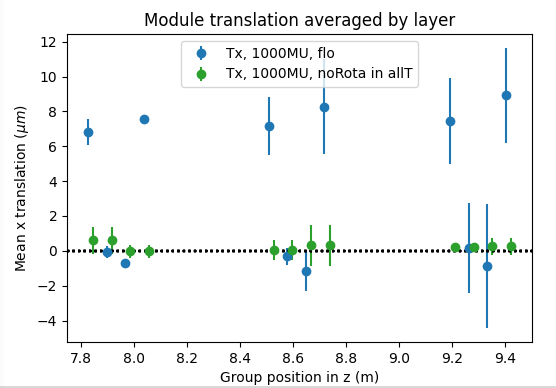
\includegraphics[width=0.8\textwidth]{plots/june_21/Tx_noRota_allT_1000MU.png}
  \caption{comparison of different configurations without rotational constraints in every station, magnet up and 1000 events. plotted is translation in x versus global z.}
  \label{fig:june_2}
\end{figure}

\begin{figure}
  \centering
  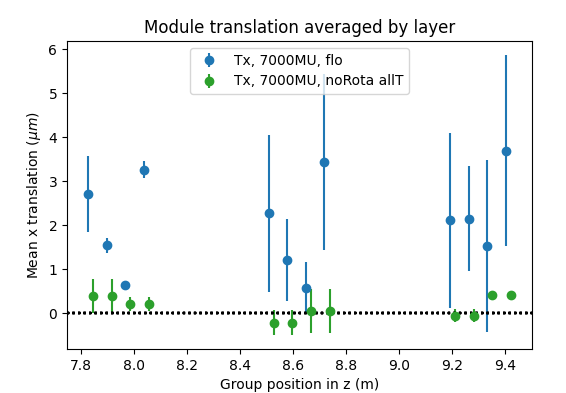
\includegraphics[width=0.8\textwidth]{plots/june_21/Tx_noRota_allT_7000MU.png}
  \caption{comparison of different configurations without rotational constraints in all stations, magnet up and 7000 events. plotted is x translation versus global z.}
  \label{fig:june_2}
\end{figure}

maybe show this plot \ref{fig:june_3}
\begin{figure}
  \centering
  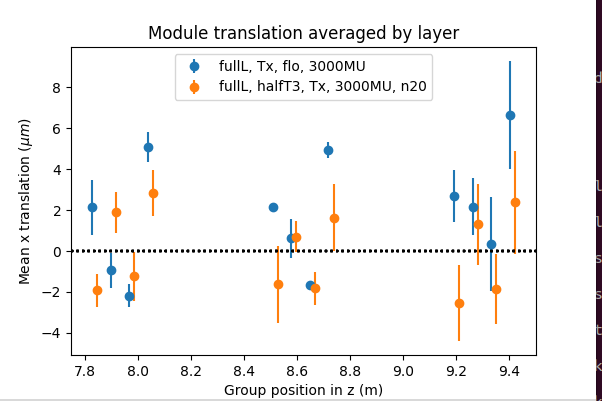
\includegraphics[width=0.8\textwidth]{plots/june_21/allT_halfT3_n20_Tx.png}
  \caption{analysed 20 iterations for x translation behavior (look up exact constraints and dofs)}
  \label{fig:june_3}
\end{figure}

\begin{figure}
  \centering
  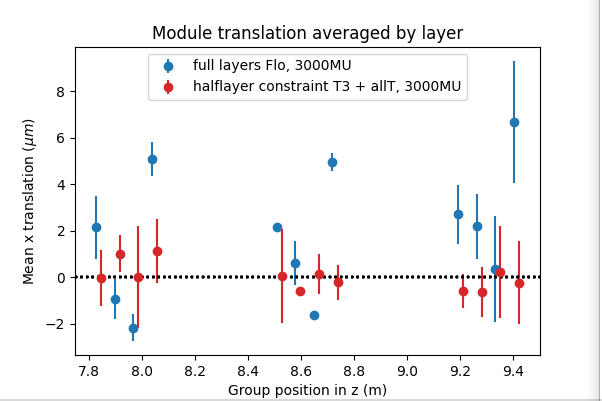
\includegraphics[width=0.8\textwidth]{plots/june_21/allT_halfT3_Tx_vs_Flo.png}
  \caption{halflayer constraints and full layer constraint, very strict (look up exact constraints and dofs)}
  \label{fig:june_4}
\end{figure}

the figure in \ref{fig:june_4} shows that very strict Tx constraints make Tx look better but when comparing to Tz as we can see in figure \ref{fig:june_5}
\begin{figure}
  \centering
  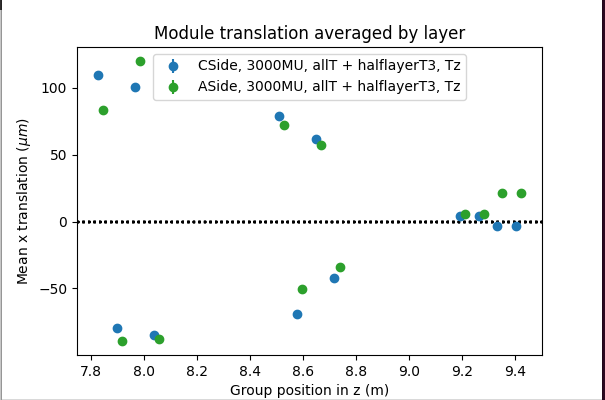
\includegraphics[width=0.8\textwidth]{plots/june_21/CA_allT_halfT3_Tz.png}
  \caption{compare C-Side to A-Side for Translation in z direction. (look up exact constraints and dofs)}
  \label{fig:june_5}
\end{figure}
a clear layer separation is visible. because of the many constraints that are applied to T3, a compensation is happening in the other two stations.

\begin{figure}
  \centering
  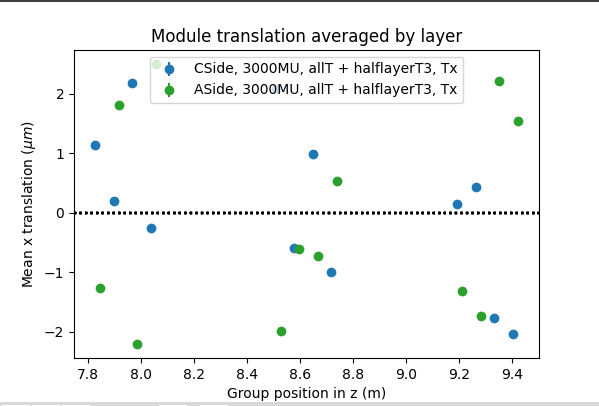
\includegraphics[width=0.8\textwidth]{plots/june_21/CA_allT_halfT3_Tx.png}
  \caption{compare C-Side to A-Side for Translation in x direction. (look up exact constraints and dofs)}
  \label{fig:june_6}
\end{figure}

Looking at figure \ref{fig:june_6}, the last two layers in station 3 are seperation from the first two. Especially the last station should be fixed around zero with the constraints added. The sum of all translations should be zero with each individual layer movement being small.

%\subsection{july plots}

test 3:
\begin{figure}
  \centering
  \begin{subfigure}[b]{0.3\textwidth}
    \centering
    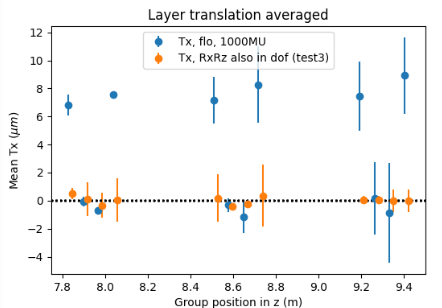
\includegraphics[width=\textwidth]{plots/july_28/Tx.png}
    \caption{Tx versus global z.}
  \end{subfigure}
  \hfill
  \begin{subfigure}[b]{0.3\textwidth}
    \centering
    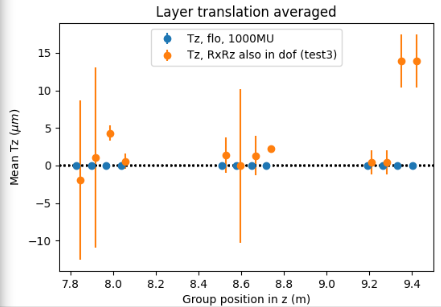
\includegraphics[width=\textwidth]{plots/july_28/Tz.png}
    \caption{Tz versus global z.}
  \end{subfigure}
  \hfill
  \begin{subfigure}[b]{0.3\textwidth}
    \centering
    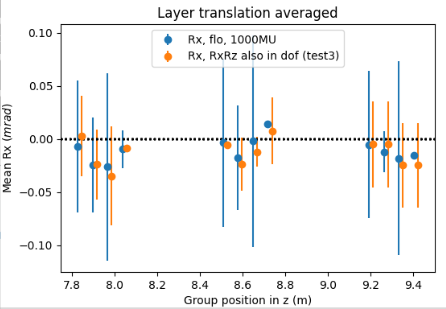
\includegraphics[width=\textwidth]{plots/july_28/Rx.png}
    \caption{Rx versus global z.}
  \end{subfigure}
  \caption{Testing a configuration versus florians changes.}
\end{figure}

%\subsection{august plots}


%%% layout %%%
%\section{Null tests and optimization of alignment parameters}
%\section{\texorpdfstring{$\chi^2$}{chi2} analysis}
%\section{Misalignment tests}
